\chapter{Two Dimensional Stochastic Case}\label{chap:twod-stochastic}

With uncertainty in the coefficients the stochastic version of Laplace's
Equation in two dimensions we will consider is:

\begin{equation}\label{eq:twod-stochastic}
      -\nabla\cdot\left[a(\v{x};\omega)\cdot\nabla u(\v{x};\omega) \right]
      = f(\v{x})\, \v{x} \in D \, \omega \in \Omega
\end{equation}

where we take $D = [-1, 1] \times [-1, 1]$, $\Omega$ is a probability space and
we impose a homogeneous Dirichlet condition on the boundary which we will
denote $\Gamma$. As with the previous stochastic case we will be following a
similar process to the original two dimensional case in order to discretise the
physical space. Then following methods outlined in \cite{general-poly-chaos} to
construct a finite dimensional approximation to elements in the probability
space.

\section{Weak Formulation}

In order to obtain the weak formulation we take the inner product of
\myref{eq:twod-stochastic} with a function $w$ from a \textit{test space} $W$
and in this sense the weak solution is given by a function $u$ from our
\textit{trial space} $V$ which satisfies the resulting equation $\forall w \in
W$. As with the previous case, our test and trial spaces are given by:

\begin{equation}
    \begin{array}{c c}
        V = H^1_0(D) \otimes L^2(\Omega) &
        W = H^1_0(D) \otimes L^2(\Omega)
    \end{array}
\end{equation}

where $H^1_0(D)$ is as defined as the closure of $C_0^\infty(D)$ with respect
to the Sobolev space norm \myref{eq:twod-H1-D-norm} and $L^2(\Omega)$ as defined
in Definition \ref{eq:L2-Omega}. So multiplying through by $w \in W$ we obtain:

\begin{equation}
    -\int_{\Omega}\int_D(\nabla\cdot\left[
        a(\v{x};\omega)\cdot\nabla u(\v{x};\omega)\right]
    w(\v{x};\omega))\, d\v{x}\, d\Omega =
        \int_{\Omega}\int_Df(\v{x})w(\v{x};\omega)\, d\v{x}\, d\Omega
\end{equation}

If we apply Green's first integral identity we obtain:

\begin{equation}
    -\int_{\Omega}\left(\int_{\Gamma}\underbrace{\frac{\partial}{\partial n}
        \left[a(x;\omega)\cdot\nabla u(x;\omega)\right]}_{=0}\, d\Gamma
      -\int_D a(x;\omega)\cdot\nabla u(x;\omega)\cdot\nabla w(x;\omega)
      w(x;\omega)\, d\v{x}
  \right)\, d\Omega
\end{equation}

where the integral on $\Gamma$ is zero as $w(x;\omega)|_\Gamma = 0$. Therefore
the weak form of the problem is given by:

\begin{equation}\label{eq:twod-stochastic-wk}
    \int_{\Omega}\int_Da(x;\omega)\nabla u(x;\omega)\cdot\nabla
    w(x;\omega)\, d\v{x}\, d\Omega =
    \int_{\Omega}\int_D f(\v{x})w(x;\omega)\, d\v{x}\, d\Omega
\end{equation}

where in this sense a solution would be a function $u \in V$ which satisfies
the the above equation $\forall w \in W$

\section{Discrete Formulation}

In order to construct a finite dimensional approximation to
\myref{eq:twod-stochastic} we must discretise both the physical and probability
spaces. For the physical space, we can proceed just as we did in Chapter
\ref{chap:twod-deterministic} and construct a uniform triangulation taking
into account that the physical domain is now $[-1,1] \times [-1,1]$.

Given a parameter $N \in \mathbb{N}$ we create a
square grid with spacing $h = 1/N$, then at each of the $M := (N+1)^2$
intersections we place a node $\v{x}_i$, $i \in \{0,\ldots, M\}$. Finally we
can split each grid square into 2 triangular elements $T_k$ using the diagonal
of negative slope. Which we can now use to define the discretisation:

\[
    \mathcal{T}_h = \bigcup_{k=1}^{2N^2}T_k
\]

Upon which we can define a finite dimensional subspace of $H^1_0(D)$:

\begin{equation}
    (H^1_0(D))^h = \{v \in H^1_0(D): v \text{ is linear on } T_k,\ i \in \{0, \ldots, 2N^2\},
                      v \text{ is continuous on } D\}
\end{equation}

Just as in the deterministic case we can use the `hat functions' as our basis
and define each $\phi_i$ associated with a node $\v{x}_i$ in terms of the
reference function \myref{eq:two-d-ref-basis-fn} as such
$\phi_i(\v{x}) = \Phi(\v{x} - \v{x}_i)$. Then we can approximate as follows:

\begin{equation}\label{eq:twod-stochastic-f-approx}
    f(\v{x}) \approx \sum_{j=0}^Mf_j\phi_j(\v{x})
\end{equation}

where $f_j = f(\v{x}_j)$. This also allows us to approximate the solution
process $u^h$ as follows:

\begin{equation}
    u^h(\v{x};\omega) = \sum_{j=0}^Mu_j(\omega)\phi_j(\v{x})
\end{equation}

where we now have a finite dimensional representation for $u$ in the physical
space but we also need a discrete representation for $u$ in the probability
space.

\subsection{Polynomial Chaos}

As in the one dimensional case in Chapter \ref{chap:oned-stochastic} we will
use members from the \textit{Askey Scheme} of Orthogonal Polynomials to form a
basis which spans the probability space. In this particular project we will be
focusing on a uniform randon process, hence we will be making use of the
\textit{Legendre Polynomials} to obtain an approximation to the solution process
$u$.

The Legendre Polynomials obey the following orthogonality relation:

\begin{equation}
    \expect{\chi_s\chi_t} = \expect{\chi_s}^2\delta_{st}
\end{equation}

With an appropriate basis chosen we can define a finite dimensional subspace of
the probability space $L^2(\Omega)$:

\begin{equation}
    (L^2(\Omega))^P = span\{\chi_1,\ldots,\chi_P\}
\end{equation}

where $P = (d + p)!/d!p!$ and $d$ denotes the dimensionality of the
approximation and $p$ represents the highest degree of polynomial used. Then we
can write the solution process as follows:

\begin{equation}\label{eq:twod-stochastic-uhp}
    u^{h,P}(\v{x};\omega) = \sum_{j=0}^M\sum_{s=0}^Pu_{j,s}
        \chi_s(\xi)\phi_j(\v{x})
\end{equation}

where $u^{h,P} \in V^{h,P} = (H^1_0(D))^h \otimes (L^2(\Omega))^P$. We can also
define a similar finite dimensional subspace for the trial space $W$.
$W^{h,P} = (H^1_0(D))^h \otimes (L^2(\Omega))^P$


\subsection{Karhumen Loeve Expansion}\label{sec:twod-stochastic-kl-expand}

The KL Expansion allows us to write a second order random process as follows:

\begin{equation}
    X(\v{x};\omega) = \bar{X}(\v{x}) +
        \sum_{n=0}^\infty\sqrt{\lambda_n}\beta_n(\v{x})\xi(\omega)
\end{equation}

See Section \ref{sec:oned-stochastic-kl-expansion} for an introduction to the
KL-Expansion.

In this case we proceed in a similar fashion to the one dimensional case where
we assume that $a(\v{x};\omega)$ has the following form:

\begin{equation}
    a(\v{x};\omega) = 1 + \epsilon\kappa(\v{x};\omega)
\end{equation}

where $\epsilon < 1$ is a small parameter and $\kappa(\v{x};\omega)$ is
uniformly distributed taking values between $a$ and $b$ with mean $\mu$,
variance $\sigma^2$ with correlation function given by:

\begin{equation}
    C(\v{x}, \v{y}) =
        \sigma^2\exp{\left(-\frac{|x_1 - y_1|}{k_1} - \frac{|x_2 - y_2|}{k_2}\right)}
\end{equation}

where for simplicity we will set the correlation lengths $k_1, k_2$ to be $1$
then to find the eigenvalues/eigenfunctions means solving the following
integral equation:

\begin{equation}\label{eq:twod-stochastic-kl-eigenvalue-problem}
    \sigma^2\int_D\exp(-|x_1 - y_1| - |x_2 - y_2|)\beta_n(\v{y})\, d\v{x}
        = \lambda_n\beta_n(\v{x})
\end{equation}

However as the kernel is seperable we can reduce this two dimensional problem
to a system of one dimensional problems:

\begin{align}
    \begin{split}
        \sigma^2\int_{-1}^1\exp(-|x_1 - y_1|)\beta^1_i(y_1)\, dy_1 &= \lambda^1_i\beta^1_i(x_1) \\
        \sigma^2\int_{-1}^1\exp(-|x_2 - y_2|)\beta^2_i(y_2)\, dy_2 &= \lambda^2_i\beta^2_i(x_2) \\
    \end{split}
\end{align}

where solutions to the original problem
\myref{eq:twod-stochastic-kl-eigenvalue-problem} are given by $\lambda_n =
\lambda^1_i\lambda^2_j$ and $\beta_n(\v{x}) = \beta^1_i(x_1)\beta^2_j(x_2)$ for
each $i, j \in \mathbb{N}$. Since the domain is $[-1, 1] \times [-1, 1]$ we can
reuse our results from earlier, using a combination of Listing
\ref{code:matlab-eigen} and Listing \ref{code:python-reconstruct-eigen} to find
each of the $\lambda_i^k$, $\beta_i^k$, for $i \in \mathbb{N}$, $k \in \{1,
2\}$.

Therefore we may approximate $a(\v{x};\omega)$ by:

\begin{equation}\label{eq:twod-stochastic-kl-kappa}
    a(\v{x};\omega) \approx 1 + \epsilon\left(
        \mu + \sigma^2\sum_{l=1}^d\sqrt{\lambda_l}\beta_l(\v{x})\xi_l(\omega)
    \right)
\end{equation}

\subsection{Derivation of the Global System of Equations}

As the weak formulation \myref{eq:twod-stochastic-wk} has to hold $\forall v
\in W$ in particular it has to hold for the basis functions so by setting
$v = \chi_t\phi_i$ for each $i \in \{0, \ldots, M\}$ and $t \in \{0, \ldots, P\}$
in \myref{eq:twod-stochastic-wk}. Also including our expansions
\myref{eq:twod-stochastic-f-approx}, \myref{eq:twod-stochastic-kl-kappa} and
\myref{eq:twod-stochastic-uhp} we obtain:

\begin{align}
  \begin{split}
    \int_\Omega\int_D
    \left[1 + \epsilon\left(\mu +
  \sigma^2\sum_{l=1}^d\sqrt{\lambda_l}\beta_l(\v{x})\xi_l(\omega)\right)\right]
      &\nabla\left(\sum_{j=0}^M\sum_{s=0}^Pu_{r,s}\chi_s(\omega)\phi_j(\v{x})\right)
      \cdot\nabla\left(\chi_t(\omega)\phi_i(\v{x})\right)\, d\v{x}\, d\Omega \\
      &= \int_\Omega\int_D\left(\sum_{j=0}^Mf_j\phi_j(\v{x})\right)
        \chi_t(\omega)\phi_i(\v{x})\, d\v{x}\, d\Omega
  \end{split}
\end{align}

By the linearity of the integral and differential operator and using our
notation for the expectation \myref{eq:oned-stochastic-expect-notation} we may
write this as:

\begin{align}\label{eq:twod-stochastic-discrete}
  \begin{split}
      \sum_{j=0}^M\sum_{s=1}^Pu_{j,s}\left[(1 + \epsilon\mu)\expect{\chi_s\chi_t}
      \left(\int_D\nabla\phi_j(\v{x})\cdot\nabla\phi_i(\v{x})\, d\v{x}\right) +
      \epsilon\sigma^2\sum_{l=1}^d\sqrt{\lambda_l}\expect{\xi_l\chi_s\chi_t}
      \left(\int_D\beta_l(\v{x})\nabla\phi_j(\v{x})\cdot\nabla\phi_i(\v{x})\, d\v{x}\right)\right] \\
      \expect{\chi_t}\sum_{j=0}^Mf_j\left(\int_D\phi_j(\v{x})\phi_i(\v{x})\, d\v{x}\right)
  \end{split}
\end{align}

for each $j \in \{0,\ldots,M\}$ and each $t \in \{1, \ldots, P\}$. Similarly to
the deterministic case, due to the homogeneous boundary condition in
\myref{eq:twod-stochastic} we can remove the terms associated with the boundary
nodes. Then by defining the $i$-th, $j$-th component of the matrix $A_{s,t}$ to
be the terms in the square brackets of \myref{eq:twod-stochastic-discrete} and
defining the $i$-th, $j$-th component of the matrix $M_t$ to be the bracketed
terms on the right hand side, we obtain the following matrix equation:

\begin{equation}
    \sum_{j=1}^{(N-1)^2}\sum_{s=1}^P(A_{s,t})_{i,j}u_{s,j} =
    \sum_{j=0}^M(M_t)_{i,j}f_j
\end{equation}

for $i \in \{1, \ldots, (N-1)^2\}$ and $t \in \{1,\ldots,P\}$. This defines a
$(N-1)^2P \times (N-1)^2P$ system of linear equations $A\v{u} = M\v{f}$ in
which the global stiffness matrix $A$ takes the following block form:

\begin{equation}
    A = \left[\begin{array}{c c c}
        A_{1,1} & \cdots & A_{1,P} \\
        \vdots & & \vdots \\
        A_{P,1} & \cdots & A_{P,P}
    \end{array}\right]
\end{equation}

where $A_{s,t}$ are $(N-1)^2 \times (N-1)^2$ matrices. Similarly the global
mass matrix $M$ takes the block form:

\begin{equation}
    M = \left[\begin{array}{c}
            M_1 \\ \vdots \\ M_P
    \end{array}\right]
\end{equation}

where $M_t$ are $(N+1)^2 \times (N-1)^2$ matrices.

\section{Constructing the Global System}

In order to construct the global system of equations we need to determine the
form of each of the $A_{s,t}$ and $M_t$ matrices.

\subsubsection{The Global Stiffness Matrix}

\subsubsection{Matrices on the Diagonal}

Setting $s = t$ in \myref{eq:twod-stochastic-discrete} we obtain the following:

\begin{equation}
    A_{s,s} = \sum_{j=1}^{(N-1)^2}\left(
(1 + \epsilon\mu)\expect{\chi_s^2}
      \int_D\nabla\phi_j(\v{x})\cdot\nabla\phi_i(\v{x})\, d\v{x} +
      \epsilon\sigma^2\sum_{l=1}^d\sqrt{\lambda_l}\expect{\xi_l\chi_s^2}
      \int_D\beta_l(\v{x})\nabla\phi_j(\v{x})\cdot\nabla\phi_i(\v{x})\, d\v{x}
      \right)
\end{equation}

for each $i \in \{1,\ldots,(N-1)^2\}$. Considering the term
$\expect{\xi_l\chi_s^2}$, specifically the fact that the product of the
functions $\chi^2$ and $\xi_l$ is odd and that by taking the expectation we
integrate over a symmetric domain the term vanishes. Hence the diagonal block
stiffness matrices reduce to:

\begin{equation}
    A_{s,s} = (1 + \epsilon\mu)\expect{\chi_s^2}
    \sum_{j=1}^{(N-1)^2}\left(\int_D\nabla\phi_j(\v{x})\cdot\nabla\phi_i(\v{x})\right)
\end{equation}

for each $i \in \{1,\ldots,(N-1)^2\}$. Now as the term $(1 +
\epsilon\mu)\expect{\chi_s^2}$ is deterministic and scalar, we are in the same
situation as in Chapter \myref{chap:twod-deterministic} and by setting
$a = (1 + \epsilon\mu)\expect{\chi_s^2}, \v{b} = \v{0}, c = 0$ in
\myref{eq:twod-deterministic-discrete-local} and if we follow a similar argument
outlined in Section \ref{sec:twod-deterministic-local-stiffness} we obtain the
following for for the local stiffness matrix $A^{(k)}_{s,s}$:

\begin{equation}
    A^{(k)}_{s,s} = \frac{(1 + \epsilon\mu)\expect{\chi_s^2}}{2}
    \left[\begin{array}{c c c}
        2  & -1 & -1 \\
        -1 & 1  & 0 \\
        -1 & 0  & 1
    \end{array}\right]
\end{equation}

Then by proceeding with an argument similar to Section
\ref{sec:twod-global-stiffnes-assembly} we find that the non zero entries of
matrix $A^{(k)}_{s,s}$ are as shown in \myref{eq:twod-deterministic-global-stiffness}

\subsubsection{The Off Diagonal Matrices}

Now considering the case where $s \neq t$ in \myref{eq:twod-stochastic-discrete}
we obtain:

\begin{equation}
    A_{s,t} = \sum_{j=1}^{(N-1)^2}\left(
(1 + \epsilon\mu)\expect{\chi_s\chi_t}
      \int_D\nabla\phi_j(\v{x})\cdot\nabla\phi_i(\v{x})\, d\v{x} +
      \epsilon\sigma^2\sum_{l=1}^d\sqrt{\lambda_l}\expect{\xi_l\chi_s\chi_t}
      \int_D\beta_l(\v{x})\nabla\phi_j(\v{x})\cdot\nabla\phi_i(\v{x})\, d\v{x}
      \right)
\end{equation}

for each $i \in \{1,\ldots,(N-1)^2\}$. Note that by the orthogonality
relation for the stochastic basis vectors $\expect{\chi_s\chi_t} =
\expect{\chi_s^2}\delta_{st}$ the first term vanishes and we have:

\begin{equation}
    A_{s,t} = \sum_{j=1}^{(N-1)^2}\left(\epsilon\sigma^2
    \sum_{l=1}^d\sqrt{\lambda_l}\expect{\xi_l\chi_s\chi_t}
    \int_D\beta_l(\v{x})\nabla\phi_j(\v{x})\cdot\nabla\phi_i(\v{x})\right)
\end{equation}

Now some care must be taken in this case as we now longer have a simple
coefficient as the form of the integral has changed from the deterministic
case. From Section \ref{sec:twod-deterministic-global-system} we know that we
can map each triangle in the discretised domain onto a reference triangle and
evaluate the integral in terms of \myref{eq:twod-local-basis}. So for the off
diagonal matrices the local stiffness matrix is given by:

\begin{equation}
    A^{(k)}_{m,n} =
    h^2\int_T\beta_l(\v{x})\nabla\psi_m(\v{x})\cdot\nabla\psi_n(\v{x})\, d\v{x}
\end{equation}

for each $m, n \in \{1, 2, 3\}$ and each $l \in \{1, \ldots, d\}$. Once we have
evaluated the integrals and obtained the form of the local stiffness matrices
for each value of $l$ and multiplied through by the corresponding coefficients
$\epsilon\sigma^2\sqrt{\lambda_l}\expect{\xi_l\chi_s\chi_t}$ we can assemble
the off diagonal matrix just as before in Section
\ref{sec:twod-global-stiffnes-assembly}

\subsection{The Global Mass Matrix}

As we saw in \ref{eq:twod-stochastic-discrete} the $t$-th block matrix from the
global mass matrix is given by:

\begin{equation}
    M_t = \expect{\chi_t}\sum_{j=0}^Mf_j
    \left(\int_D\phi_j(\v{x})\phi_i(\v{x})\, d\v{x}\right)
\end{equation}

for each $i \in \{1, \ldots, (N-1)^2\}$. As $\expect{\chi_t} =
\expect{\chi_t\chi_1}$ which by the orthogonality relation of the stochastics basis
vectors can be written as $\expect{\chi_1^2}\delta_{t,1}$. Hence the global
mass matrix is given by:

\begin{equation}
    M = \left[\begin{array}{c}
            M_1 \\ \v{0} \\ \vdots \\ \v{0}
    \end{array}\right]
\end{equation}

and as $\expect{\chi_1^2} = 1$, $M_1$ is exactly the global mass matrix we found
for the previous deterministic problem with non zeros entries given as shown in
\myref{eq:twod-deterministic-global-mass}


\paragraph{Note:}

As with the previous stochastic case that the shape of the global mass matrix
is due to the fact that we have considered a fully deterministic $f$ on the
right hand side of \myref{eq:twod-stochastic}. If we introduced some uncertainty
on the right hand side then we would be in a similar situation to the sitffness
matrix where we would have a square block matrix with non zero entries down the
diagonal.

\section{Example Problems and Results}

As stated in Section \ref{sec:twod-stochastic-kl-expand} we assume that the
diffusion coefficient can be written as $a(\v{x};\omega) = 1 +
\epsilon\kappa(\v{x};\omega)$. Taking $\mu = 1$ and the right hand side of the
equation to be $f(\v{x}) = 2\pi^2\sin{(\pi x)}\sin{(\pi y)}$ as in the
deterministic case we now consider a perturbed version of the problem. We solve
the system with combinations of the following values of $\epsilon$, $d$ and
$p$:

\begin{equation*}
    \begin{array}{c c c}
        \epsilon \in \{1, 0.1, 0.01\} &
        d \in \{1, 2\} &
        p \in \{1, 2, 3\}
    \end{array}
\end{equation*}

The code which solves these problems is detailed in Listing
\ref{code:twod-stochastic-setup}.

\subsection{Post Processing the Solution}

Now that we have our approximation to the solution process $u^{h,P}$ we can ask
questions such as what is the mean and variance of the process in the domain.

\subsubsection{Calculating the Mean}

The mean is simply the expected value of the solution process:

\begin{align}
  \begin{split}
    \mathbb{E}\left[u^{h,P}\right] = \expect{u^{h,P}}
      &= \int_\Omega\sum_{j=0}^M\sum_{s=1}^Pu_{j,s}\phi_j(\v{x})\chi_s(\omega)\, d\Omega \\
      &= \sum_{j=0}^Mu_{j,s}\phi_j(\v{x})\sum_{s=1}^P\int_\Omega\chi_s(\omega)\, d\Omega \\
      &= \sum_{j=0}^Mu_{j,1}\phi_j(\v{x})
  \end{split}
\end{align}

where due to the orthogonality relation of the stochastic basis vectors all the
stochastic terms with $s \in \{2, \ldots, P\}$ vanish. An example plot of the
expected value of one of the solution processes can be seen in Figure
\ref{fig:twod-stochastic-mean-plots}

\begin{figure}
    \centering
    \begin{subfigure}[b]{0.65\textwidth}
        \centering
        \resizebox{\linewidth}{!}{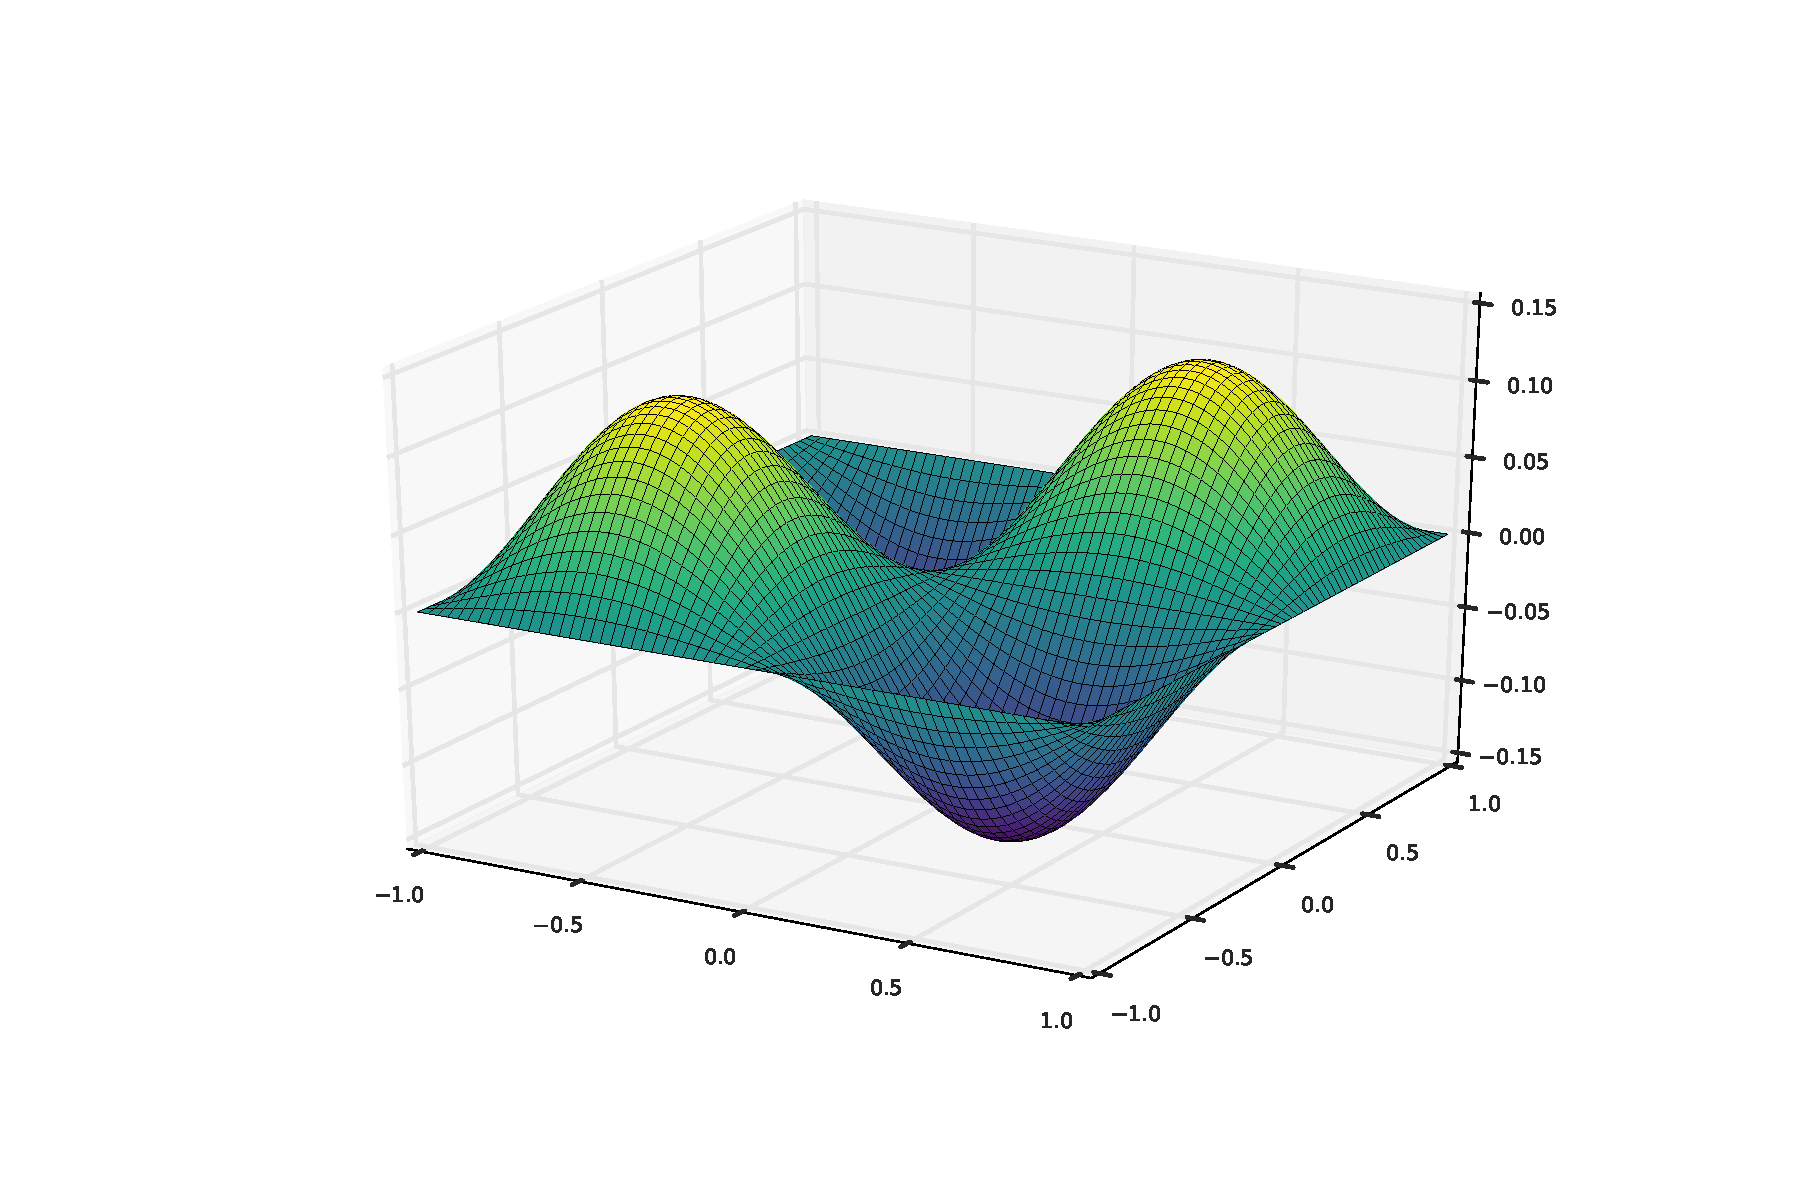
\includegraphics{img/twod-stochastic-mean-surface.pdf}}
    \end{subfigure}
    \begin{subfigure}[b]{0.55\textwidth}
        \centering
        \resizebox{\linewidth}{!}{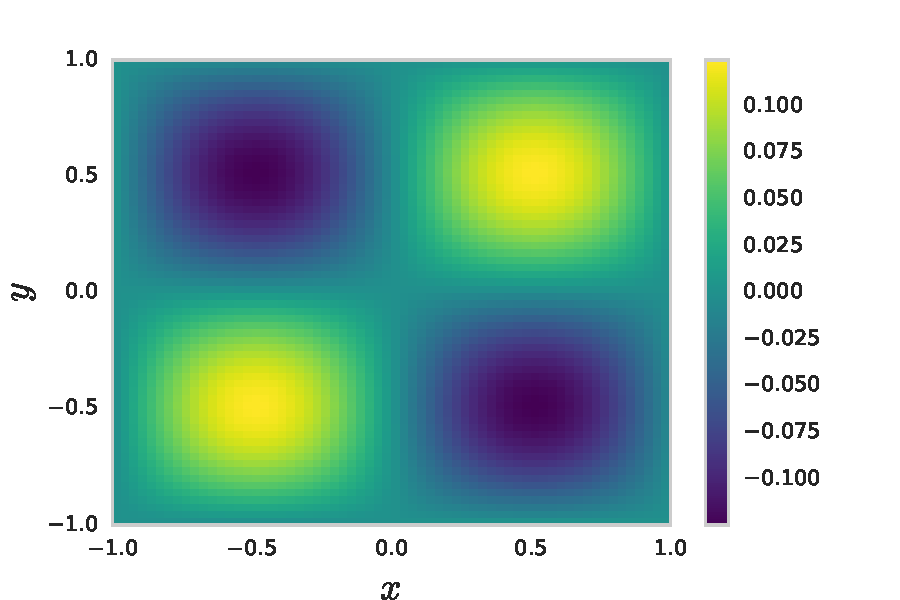
\includegraphics{img/twod-stochastic-mean-heat.pdf}}
    \end{subfigure}
    \caption{Example plot of the mean of the solution process in the case where
    $d = 1$, $p = 3$, $\epsilon = 1$, $\mu = 1$}
    \label{fig:twod-stochastic-mean-plots}
\end{figure}

\subsubsection{Calculating the Variance}

The variance of the solution process is given by:

\begin{align}
  \begin{split}
      Var(u^{h,P}) &= \mathbb{E}\left[(u^{h,P})^2\right] - (\mathbb{E}[u^{h,P}])^2 \\
        &= \int_\Omega\left(
              \sum_{j=0}^M\sum_{s=1}^Pu_{j,s}\phi_j(\v{x})\chi_s(\omega)
          \right)^2\, d\Omega - \left(\sum_{j=0}^Mu_{j,1}\phi_j(\v{x})\right)^2 \\
          &= \int_\Omega\left(\sum_{i=0}^M\sum_{j=0}^M\sum_{s=1}^P\sum_{t=1}^P
          u_{j,s}u_{i,t}\phi_j(\v{x}\phi_i(\v{x})\chi_s(\omega)\chi_t(\omega)
      \right)\, d\Omega - \left(\sum_{j=0}^Mu_{j,1}\phi_j(\v{x})\right)^2 \\
      &= \sum_{i=0}^M\sum_{j=0}^M\sum_{s=1}^P\sum_{t=1}^Pu_{j,s}u_{i,t}
         \phi_j(\v{x})\phi_i(\v{x})\int_D\chi_s(\omega)\chi_t(\omega)\, d\Omega
         - \sum_{j=0}^M\sum_{i=0}^Mu_{j,1}u_{i,1}\phi_j(\v{x})\phi_i(\v{x})
  \end{split}
\end{align}

By the orthogonality of the stochastic basis vectors this reduces to:

\begin{align}
  \begin{split}
    Var(u^{h,P}) &= \sum_{i=0}^M\sum_{j=0}^M\sum_{s=1}^P
        u_{j,s}u_{i,s}\phi_i(\v{x})\phi_j(\v{x})\expect{\chi_s^2} -
        \sum_{i=0}^M\sum_{j=0}^Mu_{j,1}u_{i,1}\phi_j(\v{x})\phi_i(\v{x}) \\
      &= \sum_{i=0}^M\sum_{j=0}^M\sum_{s=2}^P
        u_{j,s}u_{i,s}\phi_j(\v{x})\phi_i(\v{x})\expect{\chi_s^2}
  \end{split}
\end{align}

Then by considering the support of the spatial basis functions $\phi_k$ just as
we did when constructing the mass and stiffness matrices in Sections
\ref{sec:twod-global-stiffnes-assembly} and \ref{sec:twod-mass-assembly} we can
reduce the sum in $i$ over all $M$ to a sum over $S(k)$:

\begin{equation}
    Var(u^{h,P}) = \sum_{j=0}^M\sum_{i \in S(k)}\sum_{s=2}^Pu_{j,s}u_{i,s}
        \phi_j(\v{x})\phi_i(\v{x})\expect{\chi_s^2}
\end{equation}

where $S(k) = \{k, k+1, k-1, k+N, k-N, (k+1)-N, (k-1)+N\}$ which represents the
indices of the basis functions which share some support with $\phi_k$. An
example plot of the variance can be seen in Figure
\ref{fig:twod-stochastic-variance-plots}

\begin{figure}
    \centering
    \begin{subfigure}[b]{0.65\textwidth}
        \centering
        \resizebox{\linewidth}{!}{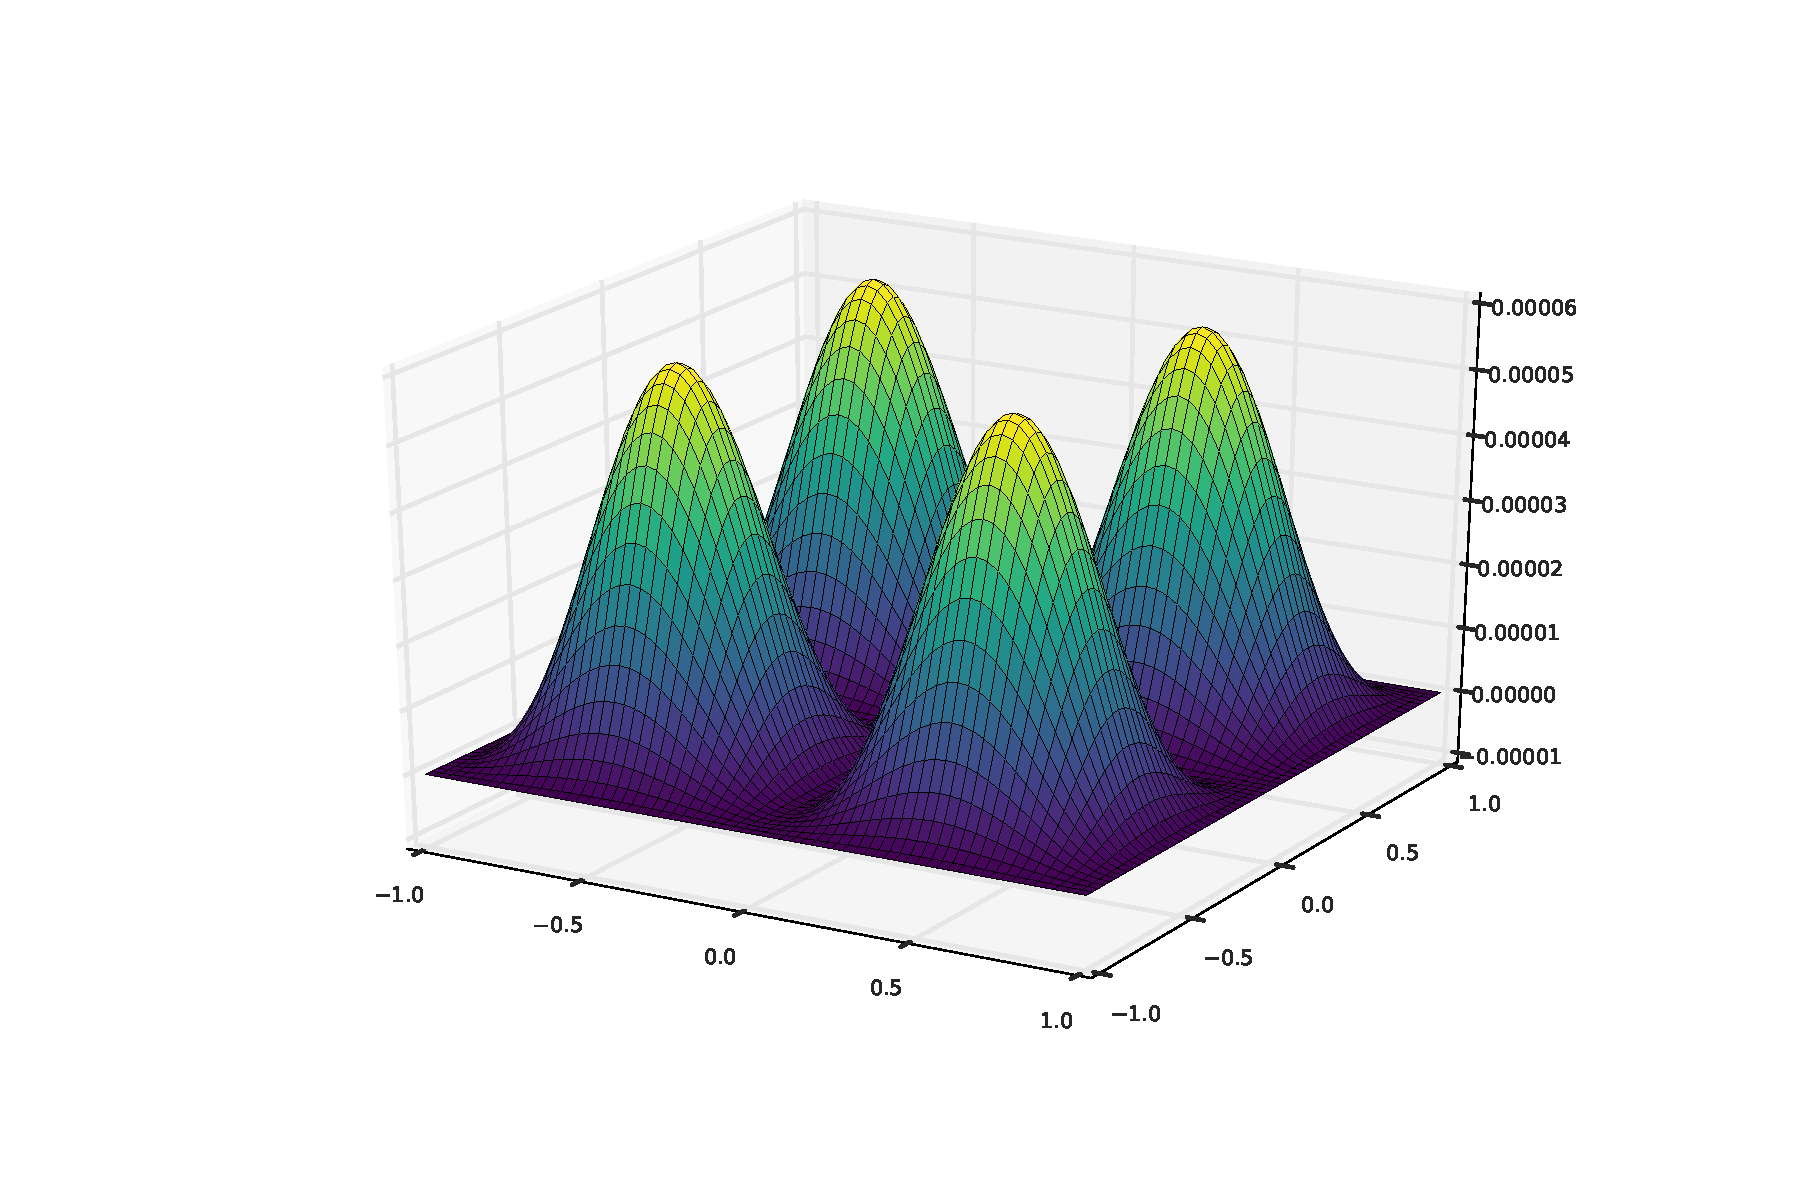
\includegraphics{img/twod-stochastic-variance-surface.pdf}}
    \end{subfigure}
    \begin{subfigure}[b]{0.55\textwidth}
        \centering
        \resizebox{\linewidth}{!}{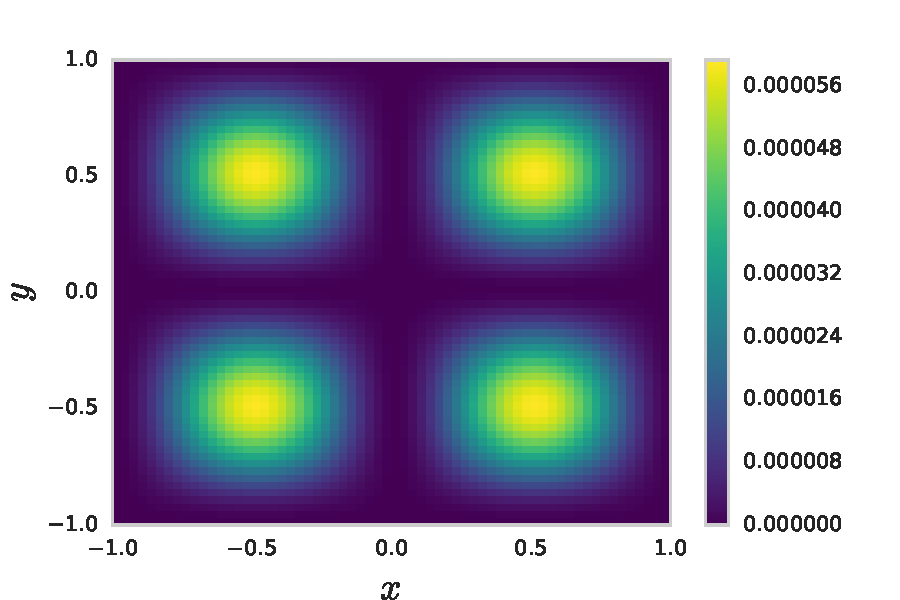
\includegraphics{img/twod-stochastic-variance-heat.pdf}}
    \end{subfigure}
    \caption{Example plot of the variance of the solution process in the case where
    $d = 1$, $p = 3$, $\epsilon = 1$, $\mu = 1$}
    \label{fig:twod-stochastic-variance-plots}
\end{figure}
